\documentclass[11pt]{article}
\usepackage[T1]{fontenc}
\usepackage[utf8]{inputenc}
\usepackage[margin=1in]{geometry}
\usepackage{lmodern,amsmath,amssymb,booktabs,graphicx,array}
\usepackage[authoryear,round]{natbib}
\usepackage{caption}
\usepackage[hidelinks]{hyperref}
\usepackage{setspace}
\setstretch{1.15}
\setlength{\emergencystretch}{2em}
\captionsetup{font=small,labelfont=bf}
\newcommand{\FamiliesN}{699}
\newcommand{\NumericN}{692}
\newcommand{\ValidN}{685}
\newcommand{\StandardizedN}{626}
\newcommand{\OrientedN}{485}
\newcommand{\RatedN}{620}
\newcommand{\BinaryMean}{-0.002}
\newcommand{\BinaryLo}{-0.041}
\newcommand{\BinaryHi}{0.037}
\newcommand{\BinaryPiLo}{-0.598}
\newcommand{\BinaryPiHi}{0.594}
\newcommand{\BinaryN}{335}
\newcommand{\BinaryAllN}{433}
\newcommand{\BinaryI}{97.2}
\newcommand{\BinaryMedianAbs}{0.067}
\newcommand{\BinarySignificant}{35.8}
\newcommand{\BinaryMissingLo}{-0.084}
\newcommand{\BinaryMissingHi}{0.064}
\newcommand{\BinarySelectionAbs}{0.085}
\newcommand{\BinaryOrientedAbs}{0.064}
\newcommand{\BinaryEggerP}{0.877}
\newcommand{\ContinuousMean}{0.011}
\newcommand{\ContinuousLo}{-0.018}
\newcommand{\ContinuousHi}{0.041}
\newcommand{\ContinuousPiLo}{-0.280}
\newcommand{\ContinuousPiHi}{0.302}
\newcommand{\ContinuousN}{150}
\newcommand{\ContinuousAllN}{193}
\newcommand{\ContinuousI}{99.2}
\newcommand{\ContinuousMedianAbs}{0.046}
\newcommand{\ContinuousSignificant}{51.3}
\newcommand{\ContinuousMissingLo}{-0.045}
\newcommand{\ContinuousMissingHi}{0.088}
\newcommand{\ContinuousSelectionAbs}{0.070}
\newcommand{\ContinuousOrientedAbs}{0.040}
\newcommand{\ContinuousEggerP}{0.386}
\newcommand{\QualityN}{620}
\newcommand{\QualityR}{0.144}
\newcommand{\QualityAdjR}{0.102}
\newcommand{\QualityPrecision}{-0.644}
\newcommand{\QualityPrecisionSE}{0.205}
\newcommand{\QualityDesign}{1.216}
\newcommand{\QualityDesignSE}{0.506}
\newcommand{\QualityRobustness}{-2.164}
\newcommand{\QualityRobustnessSE}{1.090}
\newcommand{\QualityOfficial}{2.694}
\newcommand{\QualityOfficialSE}{1.359}
\newcommand{\QualityAssumption}{-3.811}
\newcommand{\QualityAssumptionSE}{1.979}
\newcommand{\PrecisionDoubling}{-0.446}
\newcommand{\DuplicateN}{8}
\newcommand{\ComparableDuplicateN}{6}
\newcommand{\BinaryStrictMean}{0.019}
\newcommand{\BinaryStrictLo}{-0.027}
\newcommand{\BinaryStrictHi}{0.064}
\newcommand{\BinaryStrictN}{212}
\newcommand{\OriginalOrientedN}{299}
\newcommand{\NewlyOrientedN}{194}
\newcommand{\ReversedDirectionN}{1}

\title{Automated Policy Evaluation and the Interpretation of Evidence\\[6pt]
\large A Meta-Analysis of Project APE}
\author{Diego Gonz\'alez-Gonz\'alez\thanks{Draft prepared with AI assistance. The analysis summarizes reported estimates and automated annotations. It does not independently replicate the underlying policy evaluations.}}
\date{October 2, 2026}
\begin{document}
\maketitle
\begin{abstract}
Automated research can produce policy evaluations faster than their substantive validity can be assessed. I examine what can be learned from the standardized estimates reported by Project APE, an autonomous research project covering several policy areas. From \FamiliesN{} paper families with a designated effect table, I construct a comparable sample of \StandardizedN{} latest-version, non-bunching evaluations with distinct table files. I distinguish binary treatment contrasts from continuous exposure slopes and code conventional favourable outcome directions using outcome-relevant source descriptions. Direction is assignable for \OrientedN{} papers. Random-effects means are \BinaryMean{} outcome standard deviations for binary treatments and \ContinuousMean{} for one-standard-deviation changes in continuous exposure, with 95\% intervals of [\BinaryLo{}, \BinaryHi{}] and [\ContinuousLo{}, \ContinuousHi{}]. Substantial heterogeneity and selective directional coverage limit their interpretation. Tournament ratings are associated with reported precision and design descriptions, but provide no independent measure of causal validity. The corpus is useful for examining the production and assessment of evidence; its pooled estimates do not establish the welfare consequences of the policies it contains.
\end{abstract}
\noindent\textit{Keywords:} policy evaluation; automated research; meta-analysis; measurement; research assessment.

\section{Introduction}\label{sec:intro}
Policy evaluation is costly partly because economists must assemble data, justify a comparison group, and determine what an estimated change means for the people affected by a policy. Automating the production of papers reduces some of these costs. It also makes the interpretation of the resulting evidence more consequential: a large number of reported estimates can enter a policy discussion before their measurement and identification have been examined. Whether this evidence supports a useful comparison across policies depends on how outcomes are defined, how treatment intensity is measured, and which evaluations enter the comparison.

I examine these issues using Project APE, an autonomous research project that produces empirical policy evaluations from public data and publishes papers, code, and supporting materials. Its coverage includes labour markets, health, environmental regulation, housing, taxation, and governance. Many papers contain a table reporting a standardized estimate and its standard error. This common reporting format provides a starting point for comparing the distribution of reported results. It does not make the underlying policies, outcomes, or identifying assumptions equivalent.

The distinction matters even before a pooling estimator is chosen. For binary treatments, the reported standardized estimate divides a treatment coefficient by the standard deviation of the outcome. For continuous treatments, it also multiplies the coefficient by the standard deviation of exposure. The first quantity describes a discrete treatment contrast; the second describes a slope scaled to a change in exposure that varies across samples. A positive coefficient can represent higher earnings, higher mortality, or a shift in an administrative count. These changes differ economically. Moreover, a policy may achieve a stated objective while imposing costs on the affected population. A standardized outcome change alone cannot resolve that difference.

I therefore organize the analysis around measurement and coverage. I retain one selected estimate from the latest table for each paper family, preserve unclassifiable outcome directions as missing, and summarize binary and continuous estimands separately. Directional coding uses the selected outcome, table notes, and relevant definitions from data and institutional-setting sections, excluding reported results. The coding model receives neither the estimate nor the tournament rating. I distinguish a favourable change in the measured outcome from achievement of an explicit policy objective, and from a welfare improvement that would require information on costs, other outcomes, and distributional incidence.

The public snapshot contains \FamiliesN{} paper families with the designated table filename. Of these, \NumericN{} latest tables yield a numeric standardized estimate. After checking table structure, reported uncertainty, comparability, and repeated table files, \StandardizedN{} evaluations remain in the main sample. Under the contextual coding rule, \OrientedN{} allow a favourable outcome direction to be assigned, compared with \OriginalOrientedN{} under the original notes-only setup. Remaining exclusions reveal the limits of an outcome ordering even with richer descriptions. Outcome interpretation cannot be supplied by replacing every unresolved direction with a zero, or by treating every stated policy objective as beneficial.

Within the direction-coded sample, the random-effects mean is \BinaryMean{} standard deviations for binary treatments and \ContinuousMean{} for continuous exposures. The corresponding confidence intervals include zero. These averages coexist with wide model-based prediction intervals: [\BinaryPiLo{}, \BinaryPiHi{}] and [\ContinuousPiLo{}, \ContinuousPiHi{}], respectively. They summarize a selected collection of reported outcome changes. They provide little basis for predicting the effect of a particular intervention chosen from a different setting.

Directional coverage also changes the population represented by these summaries. The median absolute estimate among binary-treatment papers without an assigned direction is \BinarySelectionAbs{}, compared with \BinaryOrientedAbs{} among classified papers. The annotation setup changes both coverage and the estimated averages. Context can identify a beneficiary or clarify the definition of a variable; relaxing uncertainty restrictions can also admit poorly ordered measures. I therefore retain the original setup, stricter rules and explicit measurement safeguards in the comparison. I report these comparisons together with ranges that place no restrictions on the missing directions. The evidence does not establish that policies have no effect; it shows that a corpus-wide assertion of favourable effects requires assumptions the tables cannot verify.

I then examine how reported precision, policy descriptions, and design descriptions relate to APE's tournament ratings. These ratings are an outcome of the project's automated assessment process. Their relationship to observable paper characteristics can describe that process, even when the characteristics do not explain policy effects. The regressions use all rated papers in the comparable sample, including papers without an assigned outcome direction. Ratings are associated with greater reported precision and higher design scores, but the adjusted explanatory power is modest. Neither association identifies whether an underlying evaluation is correct.

The paper relates to two questions in empirical policy research. The first concerns how far an evaluation can inform a decision in a different setting. \citet{vivalt} documents substantial heterogeneity across impact evaluations. The APE corpus adds a prior measurement problem: before assessing transportability, the reported outcomes must be placed on an economically interpretable scale and separated by estimand. The second concerns the assessment of empirical evidence. As \citet{abadie} emphasizes, rejection of a point null need not make a result more informative than a non-rejection. The ratings analysis examines how an automated assessment covaries with precision and design descriptions, while keeping the substantive validity of the evaluations outside the observed data.

This analysis treats meta-analysis as an assessment of a reporting corpus. Conventional standardized mean differences are useful when studies measure a common construct on different scales \citep{cochrane}. Here, outcomes themselves differ, so the interpretation is narrower. A pooled coefficient is conditional on the production process, available tables, estimand definition, and directional rule. Keeping these conditions explicit allows the corpus to inform how automated evidence should be organized and assessed without turning its numerical volume into an unwarranted claim about policy success.

\section{Data and measurement}\label{sec:data}
\subsection{The research corpus}
The source is the public APE paper repository and the project's leaderboard snapshot, both accessed on October 2, 2026 (the leaderboard reports a July 1 update) \citep{ape,leaderboard}. I use the frozen repository tree to identify paper versions containing \texttt{tabF1\_sde.tex}. The analysis population is therefore the set of papers with that designated table, rather than all research produced by APE or a systematic review of the underlying policy literature. Availability of a table may itself reflect the design, outcome, or stage of revision.

Table~\ref{tab:sample} reports the sample construction. For each family, I select the latest version present among the designated tables. If that version does not contain a usable standardized estimate, I retain the exclusion in the sample accounting rather than substitute an earlier result. The filename is not sufficient to establish content: some files use ``SDE'' to mean a structured data extract or a disclosure table. Other latest tables explicitly decline to report a standardized effect. These observations cannot supply the common outcome required by the analysis.

\begin{table}[htbp]\centering\small
\caption{Sample construction}\label{tab:sample}
\setlength{\tabcolsep}{4pt}
\begin{tabular}{lr}\toprule
Stage & Paper families \\
\midrule
Latest table with designated source filename & 699 \\
Numeric standardized estimate parsed & 692 \\
Passes table validity and baseline magnitude screen & 685 \\
Comparable estimand, positive SE, non-bunching, unique table & 626 \\
Favourable outcome direction assignable & 485 \\
Rated papers in comparable sample & 620 \\
\bottomrule\end{tabular}
\par\vspace{4pt}\begin{minipage}{\textwidth}\footnotesize
\textit{Notes:} One selected estimate per latest paper-family version. Earlier versions are not substituted when the latest table lacks a usable standardized estimate. The comparable sample removes unknown estimands, bunching designs and repeated table files. Directional coding is not required for the ratings sample. The baseline magnitude screen excludes estimates exceeding five SDs; the appendix relaxes that screen.
\end{minipage}
\end{table}


The numerical extraction identifies columns by header names. It preserves escaped ampersands in outcome labels and interprets parenthesized standard errors as positive uncertainty measures. Where a classification column exists, a recognized magnitude label provides a check on column alignment. This label is not a welfare judgment or a significance test. I retain the selected row and source path so that the extraction can be traced back to the table.

The primary-row rule first selects a row in a pooled or main panel, then a main or baseline row label, and otherwise the first non-heterogeneity row with a numeric estimate. This is a reporting rule rather than an economically chosen outcome hierarchy. A paper can report several outcomes that move in different directions. Selecting one avoids counting the same evaluation several times when the covariance between its estimates is unavailable, but limits the analysis to the outcome given priority by this rule. Inferences are conditional on that selection.

Repeated files also matter. Distinct paper-family identifiers can contain identical table files. I detect these using the complete file's cryptographic hash and retain the first identifier in the sorted family list. There are \DuplicateN{} repeated latest tables; \ComparableDuplicateN{} would otherwise enter the comparable sample. This rule removes exact repetitions and does not establish that the remaining papers use independent data or examine different policies. A sensitivity analysis restores the repeated files.

\subsection{Standardization and comparability}
Let $\widehat\beta_i$ denote the coefficient selected from paper $i$, $s_{Yi}$ its reported outcome standard deviation, and $s_{Xi}$ the reported exposure standard deviation. APE uses two definitions:
\begin{equation}\label{eq:sde}
 d_i^{B}=\frac{\widehat\beta_i}{s_{Yi}}, \qquad
 d_i^{C}=\frac{\widehat\beta_i s_{Xi}}{s_{Yi}}.
\end{equation}
The superscripts $B$ and $C$ denote binary and continuous treatment. The coefficient can represent different causal contrasts, or an association, depending on the source design. Standardization does not turn an observational coefficient into a causal effect. Nor does it make a binary contrast equivalent to a one-standard-deviation change in a continuous exposure. The latter change depends on the exposure distribution in the estimation sample.

I classify the estimand using the treatment description and the declared formula in the notes. Ambiguous declarations remain outside the main pooling sample. I also exclude bunching designs, whose normalized excess-mass statistics and elasticities can differ from either quantity in equation~\eqref{eq:sde}. The baseline screen excludes absolute estimates exceeding five outcome standard deviations. This is a sensitivity choice, not a mathematical bound on standardized effects. An appendix calculation restores otherwise comparable large estimates.

Reported standard errors must be positive to enter pooling. I do not recover a standard error rounded to zero by imposing an arbitrary minimum. When the ingredients are available, I check the SDE against the declared transformation of $\widehat\beta_i$ and check its standard error against the same transformation of the coefficient's standard error. I allow a small discrepancy for rounding and report failures separately. Most continuous-treatment tables omit the exposure standard deviation, so many arithmetic identities cannot be tested. Passing a test checks internal arithmetic; it says nothing about the validity of the source comparison group.

\subsection{Outcome direction and paper characteristics}
For an outcome such as infant mortality, a reduction has a clear favourable direction for the population whose mortality is measured. For other outcomes, including fertility, cross-border banking positions, or an administrative reporting count, the direction can depend on objectives, beneficiaries, or effects outside the measured variable. I code a direction $a_i\in\{-1,1\}$ only when the notes support an interpretation. The direction-oriented estimate is $y_i=a_i d_i$. A positive value moves the selected outcome towards the coded favourable direction. If the direction is unresolved, $y_i$ is missing.

The coding uses Jev, a typed decision model supplied by TypeSafe \citep{typesafe}. Separate questions ask whether higher or lower values are conventionally favourable for the people or group described by the outcome, whether its ordering is ambiguous, and whether increasing or decreasing it is an explicit policy objective. The favourable-direction questions hold other outcomes and policy costs aside. This makes the target an interpretation of the selected measure, rather than a demand that the policy have an unambiguous net welfare effect.

The model receives the selected outcome, sanitized table notes, and up to seven relevant paragraphs from data, measurement or institutional-setting sections. Paragraph selection prioritizes the outcome's definition and population. It excludes the abstract, introduction, results and conclusion, ignores table inputs, and removes passages containing numerical effect estimates or reported uncertainty. The model sees no SDE, standard error or tournament rating. Original paper text is acquired locally from the frozen source tree; only extracted context hashes and returned annotations are redistributed. Responses are probabilities used in coding, without an independently established calibration in this corpus.

At baseline, I require a directional probability difference of at least 0.15, support of at least 0.55 for the preferred direction, and ambiguity below 0.75. I impose no additional ceiling on the opposite-direction response. These choices reduce exclusions caused by moderate confidence while retaining a minimum positive case for the assigned ordering. They were specified before examining the contextual pooled estimates. The original 0.20 margin, 0.60 support and ambiguity restrictions, including the opposite-response ceiling, remain a sensitivity comparison.

A substantive review of the contextual assignments also motivated narrow measurement safeguards. Three literal questions flag group composition, reporting or enforcement measures, and gross trading or administrative activity. A group-composition probability of at least 0.65 leaves direction unresolved because a relative share can increase without an absolute gain for its group. Reporting and activity flags require both probability of at least 0.65 and ambiguity of at least 0.40. This joint restriction avoids automatically discarding clear harmful incidents, beneficial service access or identified beneficiary burdens merely because they are observed in administrative records. The safeguards are exploratory measurement choices; their sensitivity is reported, rather than presented as a validated classifier.

Asking about both directions avoids interpreting absence of evidence for one as evidence for the other. I retain stated policy intent separately. Agreement between questions answered by the same model is a consistency check. Neither confidence thresholds nor agreement establish an optimal balance of false positives and false negatives without an external reference classification.

The resulting variable remains an outcome-direction proxy. It does not measure compensating variation, account for fiscal costs, aggregate gains and losses across people, or include all consequences of an intervention. Higher earnings for one group, for example, may be favourable for that group while leaving the policy's net welfare effect unresolved. The distinction is maintained in the interpretation of every pooled result.

A separate, frozen annotation of the table notes supplies descriptions of policy domain, instrument, design, intensity, data source, and reported tests. These covariates do not change when the directional context is expanded. Jev's design score ranges from zero to four and policy intensity from zero to three. Binary descriptions are retained as probabilities, rather than converted into certain observations. These variables characterize what the notes describe. They cannot establish that a stated test was implemented correctly or that an identification assumption holds.

I merge these records with the leaderboard's TrueSkill rating $\mu_i$, which measures performance in APE's head-to-head tournament. APE describes the judge as comparing the papers' PDFs and separately applying automated integrity checks \citep{methodology}. I use ratings only where the selected version has valid tournament matches and is not annulled. Integrity verdicts are retained for sample sensitivity. They are decisions made by the source project, not verification carried out in this meta-analysis.

\section{Empirical framework}\label{sec:methods}
\subsection{Corpus summaries}
I first examine magnitudes without requiring an outcome direction. This preserves evidence from papers whose outcomes cannot be ordered economically. I then estimate separate random-effects summaries for the direction-coded binary and continuous strata. Within a stratum, the working model is
\begin{equation}\label{eq:re}
 y_i=\theta+u_i+e_i,\qquad
 u_i\sim N(0,\tau^2),\quad e_i\sim N(0,v_i),
\end{equation}
where $\theta$ is the stratum's mean reported favourable-direction effect, $\tau^2$ is between-paper variance, and $v_i$ is the squared reported SDE standard error. Independence between papers and valid reported variances are maintained assumptions. Related policies, shared datasets, and a common research production process can violate them.

I estimate $\tau^2$ by restricted maximum likelihood \citep{viechtbauer} and weight each observation by $w_i=(v_i+\widehat\tau^2)^{-1}$. The restricted likelihood profiles out an estimated mean. Confidence intervals use modified Hartung--Knapp inference \citep{rover}. Specifically, with $k$ papers and $\widehat\theta=\sum_i w_i y_i/\sum_i w_i$, define $q=\sum_iw_i(y_i-\widehat\theta)^2/(k-1)$. The variance used for inference is $\max\{1,q\}/\sum_iw_i$, with a $t_{k-1}$ critical value. The modification prevents an unusually small residual scale from narrowing the interval below its unadjusted random-effects counterpart.

I report the heterogeneity statistic $I^2$ alongside $\widehat\tau^2$. I also report a model-based prediction interval using a $t_{k-2}$ critical value and variance $\widehat\tau^2+\widehat{\mathrm{Var}}(\widehat\theta)$. It describes dispersion under equation~\eqref{eq:re}, rather than a forecast for an arbitrary policy outside the corpus. Neither the normality of the random effects nor exchangeability across the different outcome constructs follows from standardization.

An inverse-variance fixed-effect average would impose a common effect across these outcomes and allow a few unusually precise reports to dominate. I therefore do not present it as a policy result. Equal-paper and inverse-standard-error averages provide descriptive alternatives. Their intervals use a sandwich variance that includes observed variation between papers; the uncertainty formula for a common-effect inverse-variance estimator is inappropriate for these weights.

\subsection{Descriptive regressions}
To examine which paper characteristics covary with the reported outcomes, I estimate
\begin{equation}\label{eq:reg}
 z_i=\alpha+X_i'\gamma+\delta_{m(i)}+\delta_{r(i)}+\delta_{t(i)}+\varepsilon_i,
\end{equation}
where $z_i$ is either the direction-oriented SDE or the tournament rating. The vector $X_i$ contains the log reported standard error and, in richer specifications, design, intensity, and reporting descriptions. The terms $\delta_{m(i)}$, $\delta_{r(i)}$, and $\delta_{t(i)}$ control for reported method, geographic region, and publication week. The full specification adds policy-domain controls. Rating regressions also include an estimand indicator.

Policy-outcome regressions are estimated separately by estimand. Rating regressions use all rated comparable papers and do not condition on whether the outcome direction is known. Nested specifications use a common complete sample within each table panel, so that changes in fit are not driven by changes in observations. All regressions use equal paper weights and HC3 standard errors with residual-degrees-of-freedom $t$ inference. Sparse categorical levels are grouped, and dependent columns are removed with their omission recorded.

The coefficients are descriptive associations. Policies and designs were not randomly assigned across papers, the covariates are inferred from abbreviated notes, and the rating incorporates the source project's assessment process. Noise in the dependent estimate can reduce precision; it does not by itself imply attenuation of the regression coefficients. Measurement error in the explanatory descriptions and selection into the corpus raise separate concerns. I interpret these regressions as comparisons within the reporting sample, rather than determinants of either welfare or causal validity.

\section{Reported effects across policy areas}\label{sec:results}
\subsection{Magnitude and heterogeneity}
Table~\ref{tab:distribution} and Figure~\ref{fig:magnitudes} describe all comparable estimates, including those without a favourable direction. The median absolute SDE is \BinaryMedianAbs{} for binary treatments and \ContinuousMedianAbs{} for continuous exposures. These magnitudes are expressed in outcome standard deviations, with the exposure also standardized in the continuous stratum. They cannot be translated into a common monetary benefit. Differences between strata can reflect the change in exposure being compared as well as the policy and outcome mix.

\begin{table}[htbp]\centering\small
\caption{Magnitude and reported precision}\label{tab:distribution}
\setlength{\tabcolsep}{4pt}
\begin{tabular}{lrrrrr}\toprule
Estimand & $N$ & Median $|d|$ & Mean $|d|$ & 90th pct. & $|t|>1.96$ (\%) \\
\midrule
Binary treatment & 433 & 0.067 & 0.233 & 0.563 & 35.8 \\
Continuous exposure & 193 & 0.046 & 0.196 & 0.479 & 51.3 \\
\bottomrule\end{tabular}
\par\vspace{4pt}\begin{minipage}{\textwidth}\footnotesize
\textit{Notes:} All comparable papers, including outcomes without a favourable direction. Reported standard errors are treated as data, without validating the underlying identification or inference. A nominal significance indicator is not a measure of policy success.
\end{minipage}
\end{table}

\begin{figure}[htbp]\centering
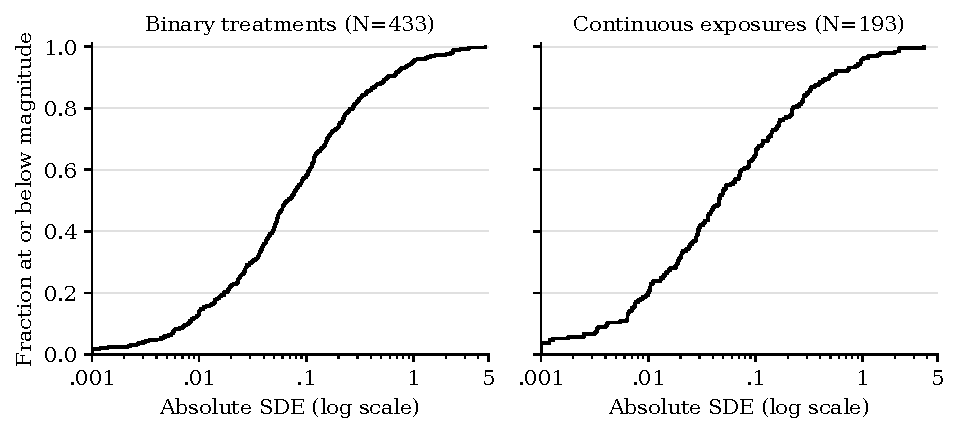
\includegraphics[width=\textwidth]{../output/figures/magnitude_cdf.pdf}
\caption{Distribution of reported magnitudes}\label{fig:magnitudes}
\begin{minipage}{\textwidth}\footnotesize\textit{Notes:} Empirical cumulative distributions for the comparable sample. The horizontal scale is logarithmic. Estimates below 0.001, including exact zeros, appear at the left boundary; all observations contribute to the cumulative fractions. The plot does not require directional coding.\end{minipage}
\end{figure}

Using the reported standard errors, \BinarySignificant{}\% of binary-treatment estimates and \ContinuousSignificant{}\% of continuous-exposure estimates have absolute normal test statistics exceeding 1.96. These fractions describe nominal significance in the tables. They do not validate the underlying standard errors, and they cannot distinguish favourable from adverse or uninterpretable changes. A sample with many statistically distinguishable outcomes can still have an average direction-oriented estimate close to zero.

Table~\ref{tab:pooled} reports the direction-coded summaries. The binary-treatment mean is \BinaryMean{} SDs across \BinaryN{} papers, with interval [\BinaryLo{}, \BinaryHi{}]. The continuous-exposure mean is \ContinuousMean{} across \ContinuousN{} papers, with interval [\ContinuousLo{}, \ContinuousHi{}]. Both intervals admit small adverse and favourable averages. As discussed by \citet{abadie}, failure to reject a zero mean does not imply that the interventions have no effects, or that an individual effect is small.

\begin{table}[htbp]\centering\small
\caption{Favourable outcome changes by estimand}\label{tab:pooled}
\setlength{\tabcolsep}{4pt}
\begin{tabular}{lrrlrrl}\toprule
Estimand & $N$ & Mean & 95\% CI & $\tau^2$ & $I^2$ (\%) & 95\% PI \\
\midrule
Binary & 335 & -0.002 & [-0.041, 0.037] & 0.091 & 97.2 & [-0.598, 0.594] \\
Continuous & 150 & 0.011 & [-0.018, 0.041] & 0.021 & 99.2 & [-0.280, 0.302] \\
\bottomrule\end{tabular}
\par\vspace{4pt}\begin{minipage}{\textwidth}\footnotesize
\textit{Notes:} REML between-paper variance and modified Hartung--Knapp inference. Positive values move the selected outcome in the coded favourable direction. These are conditional corpus summaries, not welfare or cost-benefit estimates. PI denotes a normal random-effects prediction interval; it relies on exchangeability within each corpus stratum.
\end{minipage}
\end{table}


The dispersion across papers is substantially larger than the uncertainty about either mean. The $I^2$ statistics are \BinaryI{}\% and \ContinuousI{}\%, and the prediction intervals cover outcome changes of both signs. Part of this heterogeneity can reflect differences in policies and populations. Part can arise from incompatible outcome constructs, scaling choices, imperfect source estimates, or directional classification. This decomposition cannot be identified from the reported tables alone. In particular, the size of $I^2$ should not be interpreted as a fraction of variation caused by differences in policy effectiveness.

\subsection{Policy areas and explanatory characteristics}
Figure~\ref{fig:domains} separates policy domains within each estimand. The resulting comparisons are more closely related economically than an unrestricted corpus average, but remain selected summaries of different interventions and outcomes. The classification model determines domain membership from the notes. Small cells are omitted from the figure rather than assigned an unstable estimate.

\begin{figure}[htbp]\centering
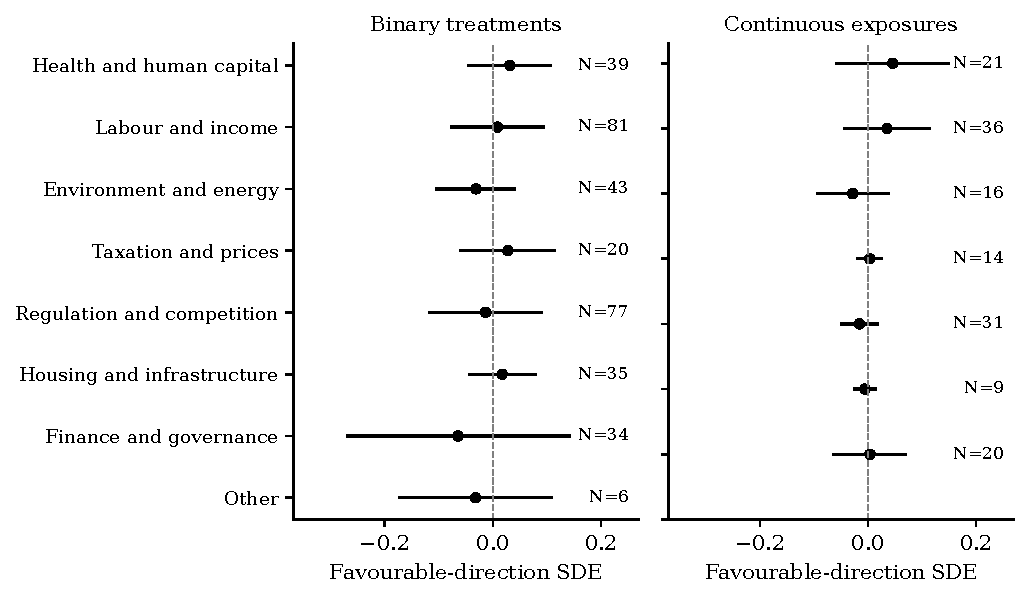
\includegraphics[width=\textwidth]{../output/figures/domains.pdf}
\caption{Direction-oriented estimates by policy domain}\label{fig:domains}
\begin{minipage}{\textwidth}\footnotesize\textit{Notes:} Points are REML means and horizontal lines are 95\% modified Hartung--Knapp intervals. Domain--estimand cells require at least five direction-coded papers. Counts appear beside each row. Differences between domains are descriptive; intervals are pointwise and do not adjust for multiple comparisons.\end{minipage}
\end{figure}

The pointwise intervals in the domain cells admit outcome changes of both signs. Differences in point estimates therefore provide a weak basis for ranking policy areas. Domain composition, outcome selection and directional coverage also differ, and the figure involves multiple comparisons. Continuous-exposure cells are particularly sensitive to the scale and distribution of the exposure variable.

Table~\ref{tab:policy_regressions} examines reported policy-outcome changes conditional on method, region, and publication week, then adds descriptions of policy and reporting characteristics. Coefficients generally remain imprecise. The richer continuous-exposure specification fits more of the observed variation, but is estimated from a smaller sample with substantially fewer residual degrees of freedom. That fit is evidence about these selected observations, not evidence that the explanatory variables identify how to design a successful intervention.

\begin{table}[htbp]\centering\small
\caption{Correlates of favourable outcome changes}\label{tab:policy_regressions}
\setlength{\tabcolsep}{4pt}
\begin{tabular}{lcccc}\toprule
 & Binary & Binary & Continuous & Continuous \\
 & (1) & (2) & (3) & (4) \\
\midrule
$\log\,\mathrm{SE}(\mathrm{SDE})$ & -0.019 & -0.015 & 0.019 & 0.034 \\
 & (0.036) & (0.036) & (0.042) & (0.042) \\
Design score & -- & 0.016 & -- & -0.083 \\
 &  & (0.050) &  & (0.060) \\
Policy intensity & -- & -0.065 & -- & 0.068 \\
 &  & (0.071) &  & (0.075) \\
Identifying-assumption test & -- & -0.062 & -- & -0.735 \\
 &  & (0.312) &  & (0.817) \\
Reports robustness & -- & -0.140 & -- & 0.245 \\
 &  & (0.122) &  & (0.290) \\
Official data source & -- & -0.075 & -- & 0.106 \\
 &  & (0.118) &  & (0.165) \\
Constant & -0.028 & 0.192 & 0.120 & 0.162 \\
 & (0.112) & (0.196) & (0.217) & (0.272) \\
\midrule Observations & 335 & 335 & 150 & 150 \\
$R^2$ & 0.057 & 0.071 & 0.069 & 0.176 \\
Adjusted $R^2$ & 0.019 & -0.004 & 0.002 & 0.040 \\
RMSE (unweighted) & 0.460 & 0.457 & 0.364 & 0.343 \\
Residual degrees of freedom & 321 & 309 & 139 & 128 \\
HC3 Wald $F$ & 0.73 & 0.43 & 0.72 & 0.71 \\
Wald $p$-value & 0.735 & 0.994 & 0.708 & 0.820 \\
Method, region, week controls & Yes & Yes & Yes & Yes \\
Policy-domain controls & No & Yes & No & Yes \\
\bottomrule\end{tabular}
\par\vspace{4pt}\begin{minipage}{\textwidth}\footnotesize
\textit{Notes:} Dependent variable is the direction-oriented SDE. Columns (1)--(2) and (3)--(4) retain common samples within each estimand. Probabilistic covariates range from zero to one; design scores from zero to four and intensity scores from zero to three. These relationships are descriptive; none identifies a determinant of policy effectiveness. HC3 standard errors in parentheses. $^{*}p<0.10$, $^{**}p<0.05$, $^{***}p<0.01$. Constant is the intercept for the omitted categorical groups; fixed effects are estimated separately. All columns use equal paper weights. Rare categorical levels (fewer than ten papers) are grouped as Other.
\end{minipage}
\end{table}


A description of an identifying-assumption test, for example, can be associated with the reported outcome because more difficult evaluations require more discussion of assumptions. Similarly, an intense intervention can target a setting where the underlying problem is more severe. The corpus offers no exogenous comparison that separates these channels. Reading the estimated coefficients as effects of improving research design or increasing policy intensity would therefore exceed what equation~\eqref{eq:reg} can identify.

\section{The assessment of research}\label{sec:ratings}
The tournament provides a second outcome: how APE's assessment process ranks a paper. Table~\ref{tab:quality_regressions} estimates the rating specifications on \QualityN{} papers. Unlike the policy-outcome table, this sample includes outcomes without an interpretable favourable direction. The common sample across columns isolates changes in specification from changes in which papers are rated.

\begin{table}[htbp]\centering\small
\caption{Correlates of tournament ratings}\label{tab:quality_regressions}
\setlength{\tabcolsep}{4pt}
\begin{tabular}{lcccc}\toprule
 & Rating & Rating & Rating & Rating \\
 & (1) & (2) & (3) & (4) \\
\midrule
$\log\,\mathrm{SE}(\mathrm{SDE})$ & -0.752$^{***}$ & -0.772$^{***}$ & -0.693$^{***}$ & -0.644$^{***}$ \\
 & (0.204) & (0.203) & (0.201) & (0.205) \\
Design score & -- & 1.078$^{**}$ & 1.165$^{**}$ & 1.216$^{**}$ \\
 &  & (0.492) & (0.507) & (0.506) \\
Policy intensity & -- & -- & 1.039$^{*}$ & 1.078$^{*}$ \\
 &  &  & (0.540) & (0.560) \\
Identifying-assumption test & -- & -- & -3.563$^{*}$ & -3.811$^{*}$ \\
 &  &  & (1.849) & (1.979) \\
Reports robustness & -- & -- & -2.272$^{**}$ & -2.164$^{**}$ \\
 &  &  & (1.073) & (1.090) \\
Official data source & -- & -- & 2.570$^{**}$ & 2.694$^{**}$ \\
 &  &  & (1.228) & (1.359) \\
Constant & 17.577$^{***}$ & 15.519$^{***}$ & 12.268$^{***}$ & 11.986$^{***}$ \\
 & (0.818) & (1.197) & (1.714) & (1.976) \\
\midrule Observations & 620 & 620 & 620 & 620 \\
$R^2$ & 0.089 & 0.098 & 0.129 & 0.144 \\
Adjusted $R^2$ & 0.063 & 0.071 & 0.097 & 0.102 \\
RMSE (unweighted) & 5.831 & 5.803 & 5.702 & 5.651 \\
Residual degrees of freedom & 602 & 601 & 597 & 590 \\
HC3 Wald $F$ & 3.24 & 3.60 & 4.10 & 3.49 \\
Wald $p$-value & $<0.001$ & $<0.001$ & $<0.001$ & $<0.001$ \\
Method, region, week controls & Yes & Yes & Yes & Yes \\
Policy-domain controls & No & No & No & Yes \\
\bottomrule\end{tabular}
\par\vspace{4pt}\begin{minipage}{\textwidth}\footnotesize
\textit{Notes:} Dependent variable is TrueSkill $\mu$. All columns use the same rated comparable papers, including those without directional coding. An estimand indicator is also included. Ratings measure the automated tournament assessment; underlying validity is not observed. HC3 standard errors in parentheses. $^{*}p<0.10$, $^{**}p<0.05$, $^{***}p<0.01$. Constant is the intercept for the omitted categorical groups; fixed effects are estimated separately. All columns use equal paper weights. Rare categorical levels (fewer than ten papers) are grouped as Other.
\end{minipage}
\end{table}


Greater reported uncertainty is associated with a lower rating. In the full specification, the coefficient on the log SDE standard error is \QualityPrecision{} rating points, with HC3 standard error \QualityPrecisionSE{}. Doubling the reported standard error is therefore associated with \PrecisionDoubling{} rating points, holding the included characteristics fixed. This association does not show that the judge correctly assesses statistical inference. Standard errors also covary with outcomes, samples, and design choices that the controls describe only imperfectly.

The coefficient on the design-description score is \QualityDesign{} points (standard error \QualityDesignSE{}). Papers whose notes are judged to describe a stronger design receive higher ratings conditional on the other included variables. The score comes from the same source prose that describes the evaluation. It cannot distinguish a credible design from a persuasive but incorrect description of that design.

Other reporting associations are less straightforward. Notes describing robustness checks have coefficient \QualityRobustness{} (standard error \QualityRobustnessSE{}), while the official-data-source probability has coefficient \QualityOfficial{} (standard error \QualityOfficialSE{}). These patterns are compatible with several explanations. Robustness discussion may occur more often when an initial estimate is fragile; official datasets may make an evaluation easier to assess. Neither explanation is independently tested here. The results should not be used to recommend omitting checks or choosing an official source solely to improve a rating.

The full specification has $R^2=\QualityR{}$ and adjusted $R^2=\QualityAdjR{}$. Most rating variation remains outside the measured characteristics. The descriptive evidence suggests that reported precision and design descriptions matter to tournament assessment, while leaving open whether the assessment tracks substantive research quality. Establishing that relationship would require independent replication and external judgments of the identification in individual papers.

\section{Sensitivity and interpretation}\label{sec:sensitivity}
\subsection{Directional coverage}
The main pooled means condition on an assigned outcome direction. This conditioning cannot be ignored. Missing directions occur when the notes omit a beneficiary or when the selected outcome represents behaviour, composition, or a trade-off that does not carry a clear favourable ordering. They can also reflect classification error or insufficient context. These sources of missingness have different economic meanings and cannot be corrected by assigning the same numerical outcome to every unresolved paper.

I vary the direction-margin and ambiguity thresholds over fifteen pairs, applying each pair to all comparable papers with the same contextual annotations and measurement safeguards. Table~\ref{tab:thresholds} reports the resulting samples and estimates separately by estimand. This exercise allows papers excluded at baseline to enter under a different rule. Restricting it to papers already classified would conceal the principal coverage margin. The thresholds are judgments about classification, rather than estimated parameters, and their sensitivity does not validate the underlying model probabilities.

The more restrictive confidence subset has a binary-treatment mean of \BinaryStrictMean{} across \BinaryStrictN{} papers, with interval [\BinaryStrictLo{}, \BinaryStrictHi{}]. The interval includes zero. Its point estimate differs from the broader sample, but neither comparison identifies what would occur among unresolved outcomes. Higher confidence can change the composition of outcomes as well as classification reliability.

Table~\ref{tab:direction_comparison} separates the original notes setup, relaxed notes rules, contextual rules and the measurement safeguards. The final contextual rule adds \NewlyOrientedN{} previously unresolved papers and changes the assigned direction of \ReversedDirectionN{} previously classified observation. Both context and question framing differ across annotation routes, so this comparison does not isolate a causal effect of supplying more text. It establishes how much the analysis population and corpus summary depend on the measurement procedure.

Source inspection illustrates why both information and restraint matter. A table labelled ``Gender Wage Gap'' measures female earnings as a percentage of male earnings in the source data section. A higher value represents a smaller earnings disparity in that setting; interpreting the label alone as an absolute gap reverses the direction. Conversely, convictions can change because courts impose punishment differently, and a group's employment share can rise when another group's employment falls. Neither variable automatically orders underlying harm or absolute gains. These examples come from an AI-assisted inspection of source definitions; they are not a representative or independent validation sample.

To make the missing-direction issue explicit, I also report finite-corpus ranges for the equal-paper average. For every unresolved paper, I allow the direction-oriented value to be either $-|d_i|$ or $|d_i|$. The resulting ranges are [\BinaryMissingLo{}, \BinaryMissingHi{}] for binary treatments and [\ContinuousMissingLo{}, \ContinuousMissingHi{}] for continuous exposures. They are algebraic bounds on the observed comparable corpus under unrestricted sign assignments, not confidence intervals and not bounds on population welfare. Their width shows how much a corpus-wide directional claim would depend on resolving the excluded outcomes.

Explicit policy objectives supply a separate interpretation. A policy can be designed to change compliance or revenue even when the beneficiary interpretation is ambiguous. Conversely, a research question asking whether employment falls does not state that lower employment is the policy's objective. I therefore retain only explicit intent in that sensitivity exercise. Its coverage is limited, and it is not a substitute for favourable outcome coding.

\subsection{Arithmetic, assessment, and dependence}
Table~\ref{tab:identities} reports internal arithmetic checks. Excluding papers that fail a test provides a limited robustness check; untestable cases remain. Source discrepancies should be resolved in the underlying evaluations before stronger substantive claims are made. Recovering a missing exposure standard deviation from the SDE being tested would make the check circular, so I do not use that procedure.

Table~\ref{tab:robustness} also removes the most precise one percent of papers, restricts the sample to the upstream clean integrity verdict, restores exact repeated table files, and relaxes the large-magnitude screen. Integrity restrictions change the sample and are not randomly assigned. A stable estimate under an automated screen cannot establish independent research validity, while a changed estimate need not identify the mechanism behind the screen's decision.

The paper-independence assumption remains a limitation after exact duplicates are removed. Different families can study related policies using overlapping datasets, and all estimates arise from a common production system. I report a country-group bootstrap for the equal-paper mean as a dependence sensitivity. Resampling geographic groups preserves dependence among papers assigned to the same country, but cannot account for every form of shared data or common model error. The usual meta-analytic intervals should be read with this limitation in mind.

Finally, I examine the association between direction-oriented standardized effects and their precision using the conventional Egger regression of the standardized normal deviate on inverse standard error \citep{egger}. The intercept-test $p$-values are \BinaryEggerP{} for binary treatments and \ContinuousEggerP{} for continuous exposures. These diagnostics do not establish that reporting is unselected. Heterogeneity, uncertain source variances, and the restriction to available tables limit their interpretation. I do not apply a mechanical correction for publication bias to this corpus, whose reporting process differs from a sample of independent published studies.

\section{Conclusion}\label{sec:conclusion}
Project APE makes a large set of automated policy evaluations available in a form that can be inspected quantitatively. I use this reporting format to examine the scale, interpretation, and assessment of its estimates. After preserving latest-version selection, distinguishing estimands, and removing exact table repetitions, the corpus exhibits substantial heterogeneity. Direction-coded averages are small and imprecise at baseline, but a more confidently classified subset yields a positive binary-treatment average. Outcomes without an assigned direction prevent extending either conclusion to the full comparable sample.

The rating regressions suggest that reported precision and descriptions of design are associated with automated research assessment. They leave the validity of the underlying evaluations unresolved. For policy use, the next step is to examine selected evaluations where the intervention, affected population, and outcome provide a coherent comparison, then verify the source data and identification. Faster production of papers increases the value of this verification. A common table format makes evidence easier to organize; an economically interpretable policy conclusion still requires information the standardized estimates do not contain.

\section*{Data availability}
The public replication package contains frozen factual table and rating extracts, cached annotation responses, all transformation and analysis code, and the manuscript sources. It reproduces the reported results offline. Source-table extraction can be rerun from the pinned public APE repository using the documented download procedure. Original paper prose and complete upstream files are not redistributed because the source snapshot does not specify an explicit redistribution licence. Full acquisition and rights information is in the package README. No independent underlying-paper replication is claimed.

\begin{thebibliography}{99}
\bibitem[Social Catalyst Lab(2026a)]{ape} Social Catalyst Lab. 2026a. \textit{Project APE papers}. GitHub repository, snapshot accessed October 2. \url{https://github.com/SocialCatalystLab/ape-papers}.
\bibitem[Social Catalyst Lab(2026b)]{leaderboard} Social Catalyst Lab. 2026b. \textit{Project APE leaderboard}. JSON snapshot accessed October 2. \url{https://ape.socialcatalystlab.org/leaderboard.json}.
\bibitem[Social Catalyst Lab(2026c)]{methodology} Social Catalyst Lab. 2026c. ``How APE Produces and Evaluates Research.'' Accessed October 2. \url{https://ape.socialcatalystlab.org/methodology}.
\bibitem[TypeSafe(2026)]{typesafe} TypeSafe. 2026. \textit{Jev 1.13.0 annotation responses}. Generated October 2 using the System One API; frozen responses in the replication package. API and question definitions: \url{https://docs.typesafe.ai/api}.
\bibitem[Deeks et al.(2024)]{cochrane} Deeks, Jonathan J., Julian P. T. Higgins, Douglas G. Altman, Joanne E. McKenzie, and Areti Angeliki Veroniki, eds. 2024. ``Analysing Data and Undertaking Meta-Analyses.'' Chapter 10, \textit{Cochrane Handbook for Systematic Reviews of Interventions}, version 6.5. Updated November 2024. \url{https://www.cochrane.org/authors/handbooks-and-manuals/handbook/current/chapter-10}.
\bibitem[Egger et al.(1997)]{egger} Egger, Matthias, George Davey Smith, Martin Schneider, and Christoph Minder. 1997. ``Bias in Meta-Analysis Detected by a Simple, Graphical Test.'' \textit{BMJ} 315 (7109): 629--634. \url{https://doi.org/10.1136/bmj.315.7109.629}.
\bibitem[R\"over, Knapp, and Friede(2015)]{rover} R\"over, Christian, Guido Knapp, and Tim Friede. 2015. ``Hartung--Knapp--Sidik--Jonkman Approach and Its Modification for Random-Effects Meta-Analysis with Few Studies.'' \textit{BMC Medical Research Methodology} 15: 99. \url{https://doi.org/10.1186/s12874-015-0091-1}.
\bibitem[Viechtbauer(2010)]{viechtbauer} Viechtbauer, Wolfgang. 2010. ``Conducting Meta-Analyses in R with the metafor Package.'' \textit{Journal of Statistical Software} 36 (3): 1--48. \url{https://doi.org/10.18637/jss.v036.i03}.
\bibitem[Abadie(2020)]{abadie} Abadie, Alberto. 2020. ``Statistical Nonsignificance in Empirical Economics.'' \textit{American Economic Review: Insights} 2 (2): 193--208. \url{https://doi.org/10.1257/aeri.20190252}.
\bibitem[Vivalt(2020)]{vivalt} Vivalt, Eva. 2020. ``How Much Can We Generalize from Impact Evaluations?'' \textit{Journal of the European Economic Association} 18 (6): 3045--3089. \url{https://doi.org/10.1093/jeea/jvaa019}.
\end{thebibliography}

\clearpage\appendix
\setcounter{table}{0}\renewcommand{\thetable}{A\arabic{table}}
\section{Directional coding sensitivity}
\begin{table}[htbp]\centering\small
\caption{Sensitivity to directional coding thresholds}\label{tab:thresholds}
\setlength{\tabcolsep}{4pt}
\begin{tabular}{rrrrlrrl}\toprule
Margin & Ambiguity & $N_B$ & Mean$_B$ & 95\% CI$_B$ & $N_C$ & Mean$_C$ & 95\% CI$_C$ \\
\midrule
0.05 & 0.60 & 325 & 0.001 & [-0.041, 0.044] & 147 & 0.005 & [-0.018, 0.027] \\
0.05 & 0.75 & 338 & 0.002 & [-0.039, 0.043] & 151 & 0.011 & [-0.018, 0.040] \\
0.05 & 0.90 & 339 & 0.002 & [-0.038, 0.043] & 151 & 0.011 & [-0.018, 0.040] \\
0.10 & 0.60 & 324 & -0.003 & [-0.043, 0.037] & 147 & 0.005 & [-0.018, 0.027] \\
0.10 & 0.75 & 337 & -0.002 & [-0.041, 0.036] & 151 & 0.011 & [-0.018, 0.040] \\
0.10 & 0.90 & 338 & -0.002 & [-0.040, 0.036] & 151 & 0.011 & [-0.018, 0.040] \\
0.15 & 0.60 & 322 & -0.003 & [-0.043, 0.037] & 146 & 0.005 & [-0.018, 0.027] \\
0.15 & 0.75 & 335 & -0.002 & [-0.041, 0.037] & 150 & 0.011 & [-0.018, 0.041] \\
0.15 & 0.90 & 336 & -0.002 & [-0.041, 0.036] & 150 & 0.011 & [-0.018, 0.041] \\
0.20 & 0.60 & 321 & -0.004 & [-0.044, 0.037] & 146 & 0.005 & [-0.018, 0.027] \\
0.20 & 0.75 & 333 & -0.003 & [-0.042, 0.036] & 150 & 0.011 & [-0.018, 0.041] \\
0.20 & 0.90 & 334 & -0.003 & [-0.042, 0.036] & 150 & 0.011 & [-0.018, 0.041] \\
0.30 & 0.60 & 314 & -0.008 & [-0.047, 0.031] & 144 & 0.006 & [-0.017, 0.029] \\
0.30 & 0.75 & 325 & -0.007 & [-0.045, 0.031] & 148 & 0.013 & [-0.017, 0.042] \\
0.30 & 0.90 & 326 & -0.007 & [-0.045, 0.031] & 148 & 0.013 & [-0.017, 0.042] \\
\bottomrule\end{tabular}
\par\vspace{4pt}\begin{minipage}{\textwidth}\footnotesize
\textit{Notes:} Each threshold pair is reapplied to all comparable papers with contextual annotations. B and C denote binary and continuous estimands. Maximum directional support must reach 0.55; there is no separate ceiling for the opposite-direction response. These thresholds are sensitivity choices, not empirically calibrated cutoffs.
\end{minipage}
\end{table}

\clearpage
\section{Alternative samples}
\begin{table}[htbp]\centering\small
\caption{Alternative samples and interpretation rules}\label{tab:robustness}
\setlength{\tabcolsep}{4pt}
\begin{tabular}{llrrl}\toprule
Estimand & Sample or rule & $N$ & Mean & 95\% CI \\
\midrule
Binary & Arithmetic screen & 326 & 0.000 & [-0.040, 0.040] \\
Binary & Direction agreement & 21 & 0.006 & [-0.072, 0.084] \\
Binary & Confident direction & 212 & 0.019 & [-0.027, 0.064] \\
Binary & Drop most precise 1\% & 331 & -0.002 & [-0.042, 0.037] \\
Binary & Clean scan & 152 & 0.009 & [-0.050, 0.068] \\
Binary & Policy intent & 27 & 0.033 & [-0.113, 0.179] \\
Binary & Include large SDEs & 336 & -0.008 & [-0.052, 0.036] \\
Binary & Include duplicate tables & 337 & -0.002 & [-0.040, 0.037] \\
Continuous & Arithmetic screen & 150 & 0.011 & [-0.018, 0.041] \\
Continuous & Confident direction & 101 & -0.004 & [-0.028, 0.021] \\
Continuous & Drop most precise 1\% & 148 & 0.012 & [-0.018, 0.041] \\
Continuous & Clean scan & 82 & -0.010 & [-0.032, 0.012] \\
Continuous & Policy intent & 5 & 0.055 & [-0.022, 0.132] \\
Continuous & Include large SDEs & 151 & 0.011 & [-0.018, 0.041] \\
Continuous & Include duplicate tables & 154 & 0.009 & [-0.020, 0.038] \\
\bottomrule\end{tabular}
\par\vspace{4pt}\begin{minipage}{\textwidth}\footnotesize
\textit{Notes:} All entries use REML and modified Hartung--Knapp inference. Clean scan is the upstream CLEAN verdict; it is not independent verification. The confidence subset requires direction margin at least 0.60 and ambiguity below 0.30. Policy intent uses explicit stated objectives and answers a different question.
\end{minipage}
\end{table}

\clearpage
\section{Arithmetic checks and alternative weights}
\begin{table}[htbp]\centering\small
\caption{Internal arithmetic diagnostics}\label{tab:identities}
\setlength{\tabcolsep}{4pt}
\begin{tabular}{lrrrrr}\toprule
Estimand & Total & SDE tested & SDE fails & SE tested & SE fails \\
\midrule
Binary & 433 & 429 & 10 & 404 & 7 \\
Continuous & 193 & 39 & 0 & 7 & 0 \\
\bottomrule\end{tabular}
\par\vspace{4pt}\begin{minipage}{\textwidth}\footnotesize
\textit{Notes:} SDE is checked against the declared standardization and SE against the same multiplier. A test is uninformative when the denominator or continuous exposure SD is unavailable. Tolerances allow 10\% relative SDE and 15\% relative SE discrepancies, with small-value floors of 0.02 and 0.0001. Counts are diagnostics, not estimates of research reliability.
\end{minipage}
\end{table}

\begin{table}[htbp]\centering\small
\caption{Descriptive averages under alternative weights}\label{tab:weights}
\setlength{\tabcolsep}{4pt}
\begin{tabular}{llrrl}\toprule
Estimand & Weight & $N$ & Mean & 95\% CI \\
\midrule
Binary & Equal & 335 & -0.013 & [-0.064, 0.038] \\
Binary & Inverse SE & 335 & -0.008 & [-0.027, 0.011] \\
Continuous & Equal & 150 & 0.028 & [-0.033, 0.089] \\
Continuous & Inverse SE & 150 & 0.006 & [-0.012, 0.023] \\
\bottomrule\end{tabular}
\par\vspace{4pt}\begin{minipage}{\textwidth}\footnotesize
\textit{Notes:} Intervals use a paper-level sandwich variance for the weighted mean, including observed between-paper variation. Country-group bootstrap ranges are reported in the machine-readable results. No fixed-effect point estimate is presented as a policy result.
\end{minipage}
\end{table}

\clearpage
\section{Annotation setup and coverage}
\begin{table}[htbp]\centering\small
\caption{Annotation setup and directional coverage}\label{tab:direction_comparison}
\setlength{\tabcolsep}{4pt}
\begin{tabular}{llrrl}\toprule
Setup and rule & Estimand & $N$ & Mean & 95\% CI \\
\midrule
Notes / strict & Binary & 210 & 0.018 & [-0.018, 0.053] \\
Notes / strict & Continuous & 89 & 0.015 & [-0.016, 0.046] \\
Notes / relaxed & Binary & 278 & -0.006 & [-0.046, 0.033] \\
Notes / relaxed & Continuous & 123 & 0.001 & [-0.029, 0.031] \\
Context / strict & Binary & 307 & -0.007 & [-0.048, 0.033] \\
Context / strict & Continuous & 139 & 0.000 & [-0.021, 0.022] \\
Context / unguarded & Binary & 366 & -0.011 & [-0.051, 0.028] \\
Context / unguarded & Continuous & 161 & 0.016 & [-0.013, 0.044] \\
Context / balanced & Binary & 335 & -0.002 & [-0.041, 0.037] \\
Context / balanced & Continuous & 150 & 0.011 & [-0.018, 0.041] \\
\bottomrule\end{tabular}
\par\vspace{4pt}\begin{minipage}{\textwidth}\footnotesize
\textit{Notes:} Notes refers to the original beneficiary questions and table notes. Context refers to outcome-relevant data/setting paragraphs and questions explicitly about conventional outcome ordering, holding other outcomes and policy costs aside. Thus both context and question framing change across routes. Strict requires margin 0.20, support 0.60, opposite support no greater than 0.40 and ambiguity below 0.60. Balanced requires margin 0.15, support 0.55 and ambiguity below 0.75, with no opposite-support ceiling. Both routes use the same estimator. Contextual guarded rules flag group composition at probability 0.65; reporting/enforcement and gross-activity flags at 0.65 additionally require ambiguity at least 0.40. Unguarded omits these safeguards. These comparisons are not classification-error estimates.
\end{minipage}
\end{table}

\end{document}
